\documentclass[openany]{book}

\usepackage[a4paper]{geometry}

\usepackage[T2A]{fontenc}
\usepackage[utf8]{inputenc}
\usepackage[english,russian]{babel}

\usepackage{graphicx}

\begin{document}

\tableofcontents

\part{Релейный конструктор}

\chapter{Введение}


\chapter{Первые эксперименты с конструктором}


\section{Модуль переключателей}

\begin{center}
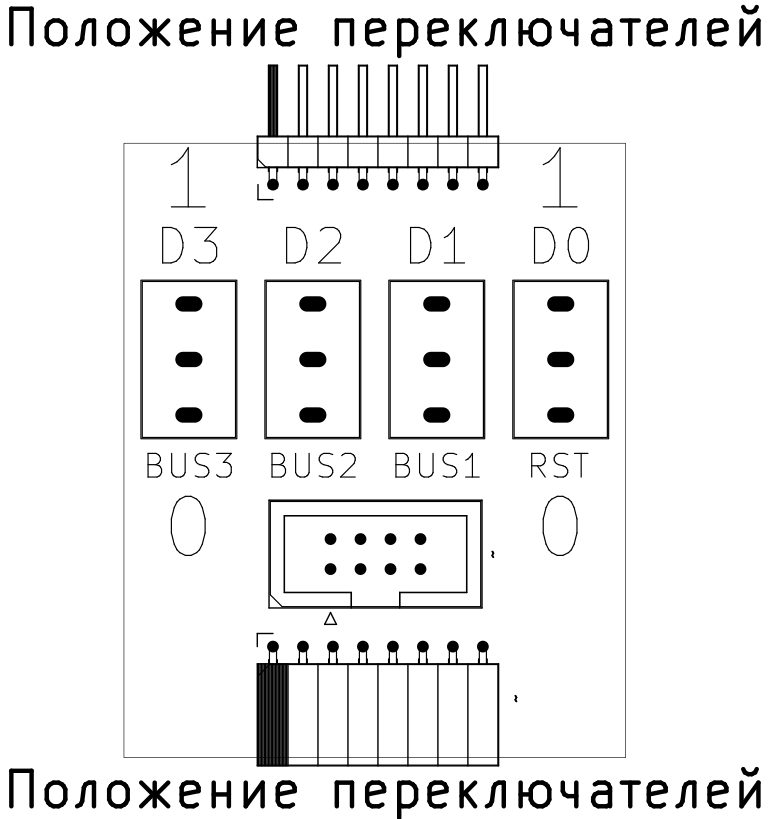
\includegraphics{boards/switches.png}
\end{center}

Модуль с тумблерами используется для ручного включения и выключения реле.
Присоединяя его к разным разъёмам, можно задавать четырёхбитное число,
либо переключать до четырёх управляющих сигналов.

Проще всего проверить работу тумблеров, подключив их к управляющей шине
регистрового модуля, в который вставлены только $4$ реле.

\subsection{Практикум}


Список модулей:
\begin{itemize}
    \item Модуль переключателей: $1$ штука
    \item Регистровый модуль как шинный формирователь: $1$ штука
\end{itemize}

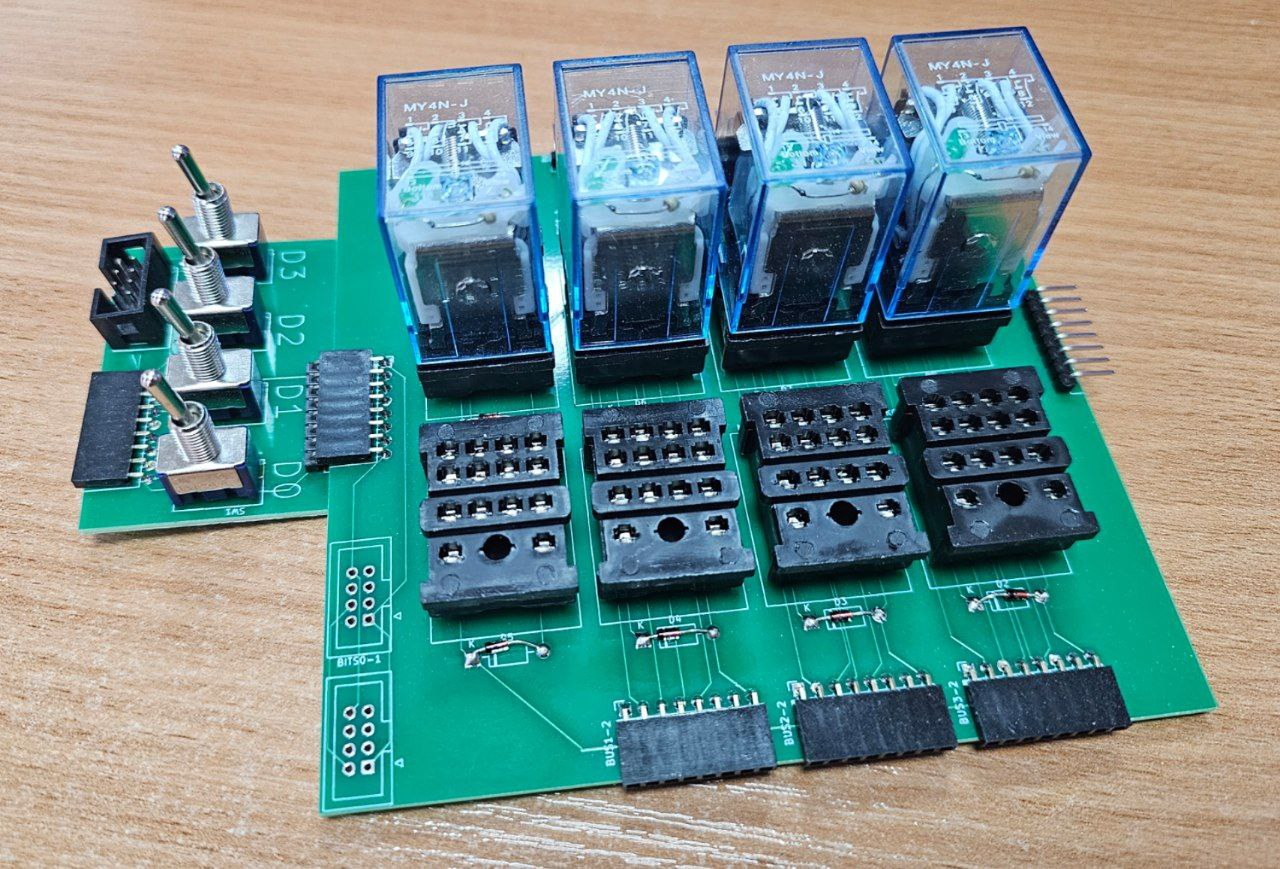
\includegraphics[width=0.5\columnwidth]{photo/switches.jpg}

\begin{enumerate}
    \item Переключать тумблеры. Убедиться, что положение одного тумблера меняет состояние одного реле.
    \item Запомнить включенное и выключенное состояния тумблера, чтобы позднее не было проблем с управлением другими схемами.
\end{enumerate}

\subsection{Задачи}

\begin{enumerate}
    \item Придумать, как соединить тумблеры для выполнения логического ИЛИ.
    \item Придумать, как соединить тумблеры для выполнения логического И.
\end{enumerate}



\chapter{Хранение и передача данных}


\section{RS-триггер}

Триггер --- это простейшее устройство для хранения одного бита информации.
Если он включен, там хранится единица, а если выключен --- хранится ноль.

Хранение одного бита можно сделать с помощью одного реле.
Если оно включается, то сохранена единица.
Чтобы это включённое состояние запоминалось, нужно организовать обратную
связь через один из контактов. Как только реле включается с помощью
входа $SET$, на его
обмотку подаётся напряжение через его же замкнутый контакт. Поэтому даже
если перестать подавать напряжение на вход $SET$, реле всё равно останется включённым:

\begin{center}
\includegraphics{schemes/trigger1.png}
\end{center}

Но если такое реле уже включилось, выключить его не получится. Единственный способ ---
это снять питание. Тогда контакты разомкнутся и при повторной подаче питания реле будет
в выключенном состоянии.

Чтобы не отключать всю схему, нужно предусмотреть отдельное реле, позволяющее
отключить питание только для этой схемы:

\begin{center}
\includegraphics{schemes/trigger2.png}
\end{center}

Теперь подав сигнал на вход $RESET$ можно сбросить триггер. И там опять окажется ноль.

Триггер с двумя входами $RESET$ и $SET$ называется RS-триггером.
На практике удобно объединить несколько таких триггеров в многобитовый регистр
и использовать для них единый сигнал сброса, сэкономив несколько реле.

\section{Шина}

Шина --- это набор проводников, объединённых общим назначением.
К этим проводникам подключаются несколько устройств для обмена сигналами.

Например, по шине данных процессор может читать или записывать данные из памяти
или жёсткого диска. Шина адреса используется для выбора определённой ячейки в памяти.
А по шине управления приходят сигналы, позволяющие отличать обращение к памяти
от обращения к диску.

Так как к шине обычно подключается больше одного входа и больше одного выхода,
необходимо изолировать лишние устройства, когда шина используется другими.
В релейном компьютере мы можем использовать для подключения к четырёхбитной шине
шинный формирователь из одного реле:

\begin{center}
\includegraphics{schemes/bus.png}
\end{center}

Когда такое реле включается, оно может соединить какое-то устройство (например, регистр)
с шиной. Подключение будет двунаправленным, поэтому с помощью этой схемы можно как
записывать данные в регистр, так и считывать оттуда.

Шинные формирователи подключаются к каждому устройству, поэтому
для передачи данных и вычислений требуется формировать множество сигналов $SELECT$.

\section{Шины в конструкторе}

В конструкторе все компоненты соединяются с помощью восьмибитных шлейфов.
В каждом из них есть питание и земля. Кроме того, большинство из таких
подключений это шина в которой от $1$ до $4$ сигналов.

Например, $4$ сигнала могут использоваться для управления модулем регистра.
Или для передачи данных из одного регистра в другой.
Каждым из таких сигналов можно управлять с помощью модуля переключателей,
соединив его с соответствующей шиной.

\section{Регистр}

Регистры внутри процессоров (или периферийных устройств)
используются для хранения данных и для проведения вычислений.
Регистры могут иметь выделенное назначение (например, хранить режим работы устройства)
или же используются почти для всего (адрес, операнд арифметических операций,
значение для ввода-вывода).

\begin{center}
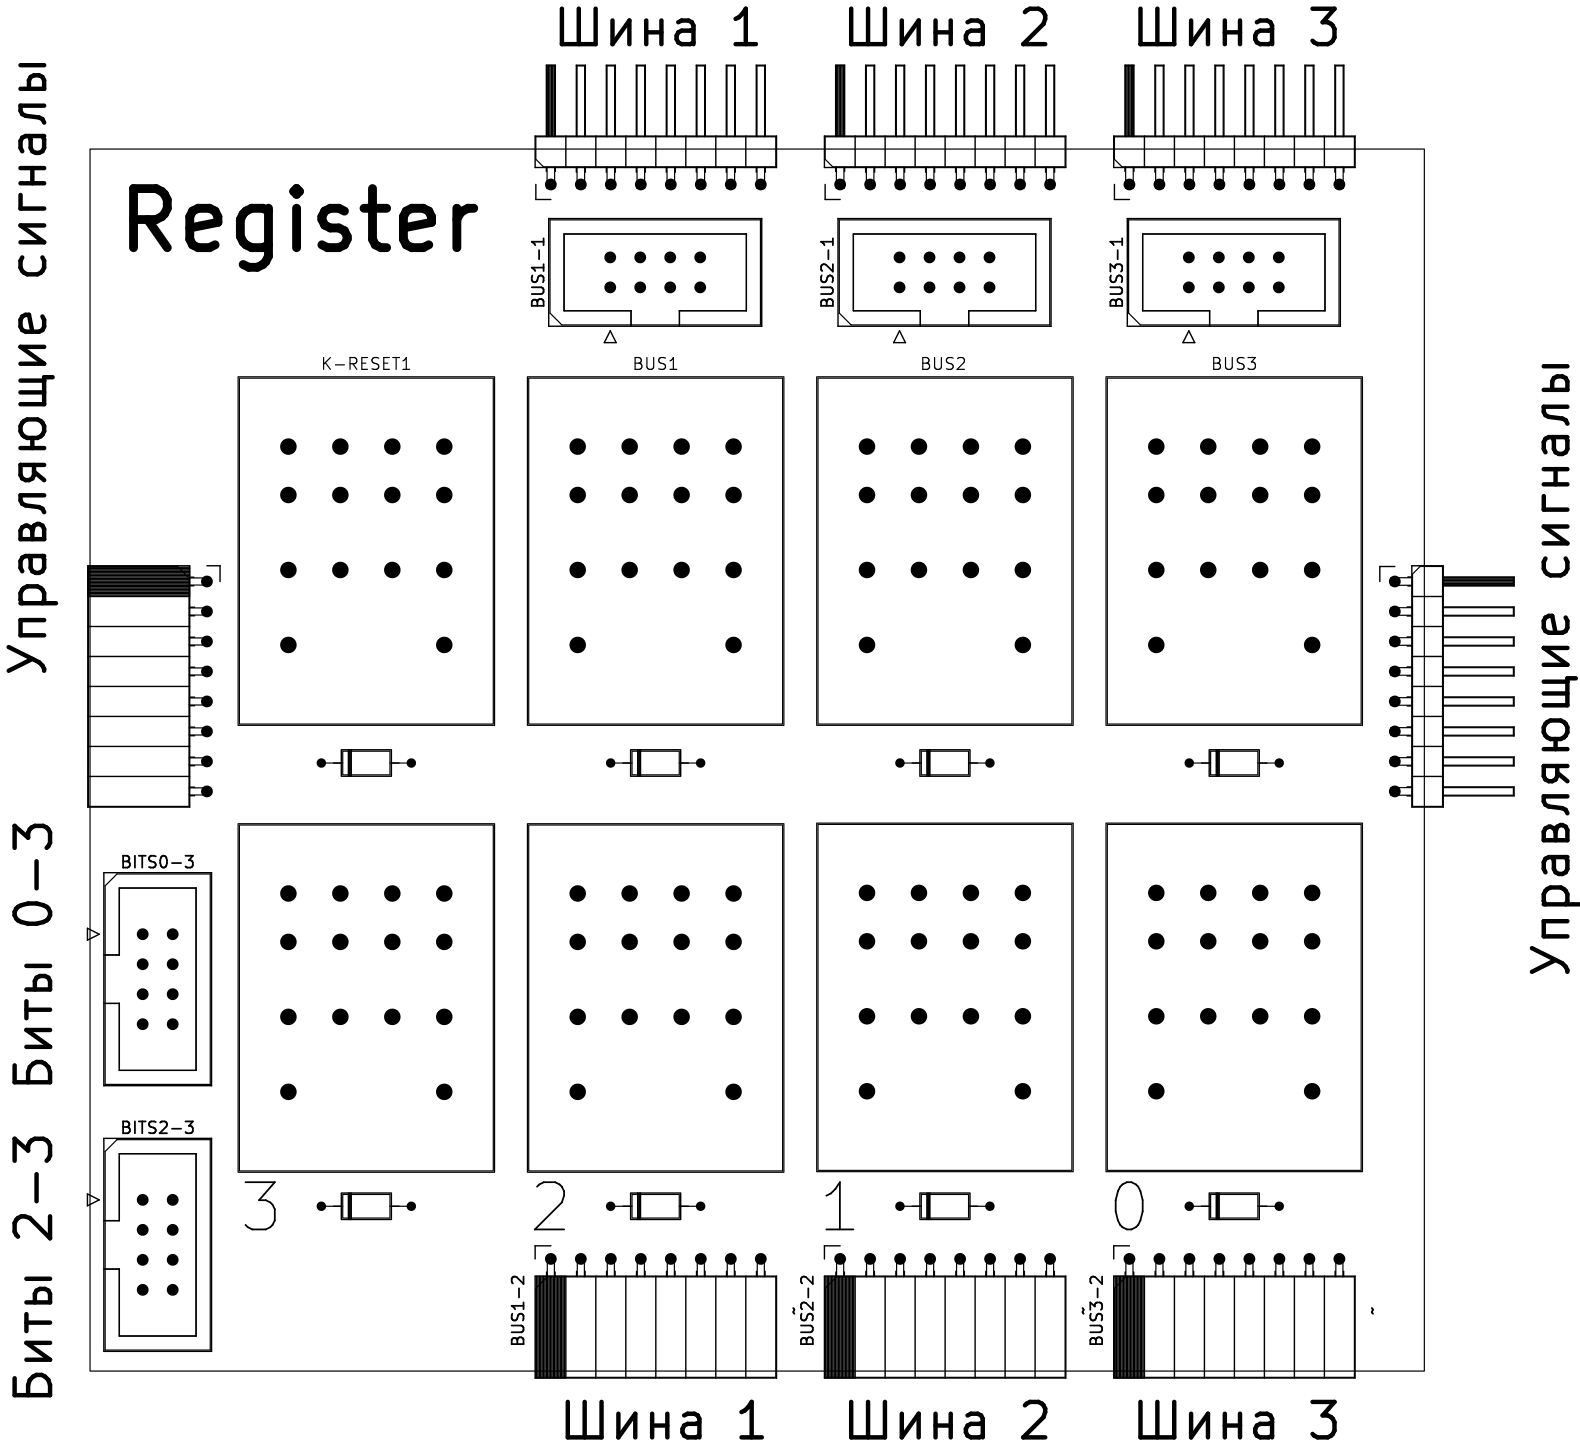
\includegraphics{boards/register.png}
\end{center}

Модуль четырёхбитного регистра состоит из четырёх реле-триггеров,
одного реле для обнуления регистра и трёх реле для подключения
к шинам данных.

Для хранения данных используются RS-триггеры, описанные выше,
но сигнал для сброса у них общий. Таким образом, записывать
данные можно только во все четыре бита сразу. Поэтому такой
модуль и реализует функции цельного регистра, а не нескольких
разрозненных RS-триггеров.

Также модуль регистра содержит три шинных формирователя.
Их можно использовать для подключения триггеров к разным устройствам
через три шины. Например, одна шина может быть предназначена
для первого операнда при вычислениях, вторая для второго операнда,
а третья для копирования данных между регистрами.

Если в модуль установить только реле шинных формирователей,
получится модуль, который может подключать четырёхбитные сигналы
(полученные из разъёма для прямого чтения значений триггеров) к одной
из выбранных шин.

Модуль регистра имеет следующие разъёмы:
\begin{itemize}
  \item Слева и справа: управляющие сигналы сброса и выборки.
        Можно подключить тумблеры
        для ручного включения сигналов. Также можно соединить несколько
        модулей регистра, чтобы управлять одним набором сигналов сразу
        для $8$, $12$ \ldots бит.
  \item Сверху и снизу: три шины данных. Реле регистра могут
        подключаться к шинам для записи или чтения данных.
  \item Дополнительные разъёмы с битами $0-3$ и $2-3$ для чтения или
        записи значения без подключения к шине.
\end{itemize}

Чтобы прочитать значение регистра нужно активировать сигнал выборки
его на нужную шину. А уже через шину сигналы поступят на вход какой-то
другой схемы.

Для записи значения в регистр нужно сначала обнулить его триггеры,
иначе запись не произойдёт в тех битах, где уже хранятся единицы.
После этого регистр подключается к нужной шине, и триггеры
защёлкивают нужное значение.

\subsection{Практикум}


Список модулей:
\begin{itemize}
    \item Модуль переключателей: $2$ штуки
    \item Регистровый модуль: $1$ штука
\end{itemize}

Протестировать работу регистра можно собрав следующую схему:

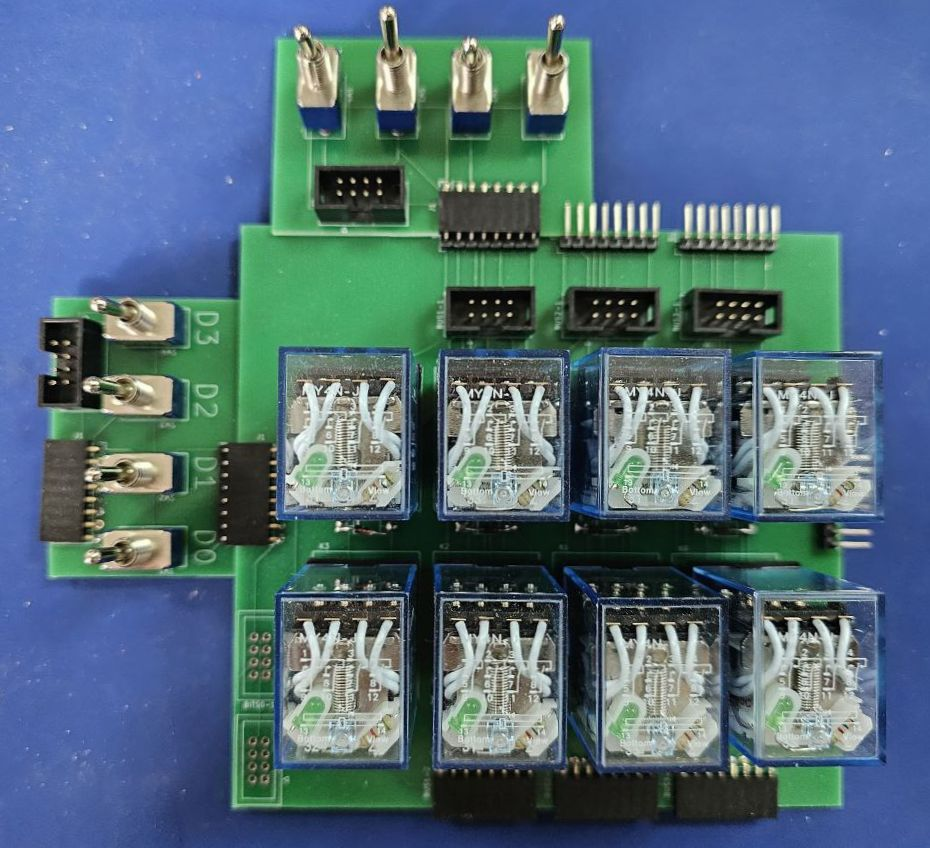
\includegraphics[width=0.5\columnwidth]{photo/register.jpg}

\begin{itemize}
  \item Тумблеры слева управляют работой регистра. Бит 0 --- обнуление, бит 1 --- выборка на шину 1.
  \item Тумблеры сверху нужны для ввода значения регистра. Когда он подключается к шине 1,
        значения, набранное на тумблерах, записывается в регистр.
\end{itemize}

\subsubsection{Регистр без шины}

\begin{enumerate}
    \item Подключить тумблеры проводом к битам $0-3$ вместо шины.
    \item Набирать значение, убедиться, что биты переключаются в $1$, но не возвращаются в $0$.
    \item Обнулить тумблеры с данными.
    \item Включить и выключить сигнал сброса. Убедиться, что значения всех битов теперь $0$.
\end{enumerate}

\subsubsection{Регистр с шиной}

\begin{enumerate}
    \item Отключить все управляющие сигналы.
    \item Набрать значение на тумблерах для данных. Убедиться, что это не влияет на регистр.
    \item Включить и выключить сигнал выборки на шину $1$. Убедиться, что данные записались в регистр.
    \item Включить и выключить сигнал сброса. Убедиться, что значения всех битов теперь $0$.
\end{enumerate}

\subsection{Задачи}

\begin{enumerate}
    \item Придумайте, как скопировать данные из одного регистра в другой, не запоминая их в голове.
\end{enumerate}


\section{Шина и регистровый файл}

Несколько регистров можно соединить в регистровый файл.
Регистровый файл --- это набор регистров. Он может быть однородным
(все регистры эквивалентны) или нет (разные регистры имеют разное назначение).

У каждого из регистров есть сигналы выборки на одну из трёх шин.
Если два регистра подключены к одной шине одновременно,
то значения одного будут копироваться в другой. Если точнее,
включённые биты включают аналогичные в другом регистре, то есть
копирование возможно в обе стороны одновременно.

Нулевые биты при этом копироваться не могут. Для записи нулей
регистр необходимо сбросить.


\subsection{Практикум}


Список модулей:
\begin{itemize}
    \item Модуль переключателей: $5$ штук
    \item Регистровый модуль: $4$ штуки
\end{itemize}

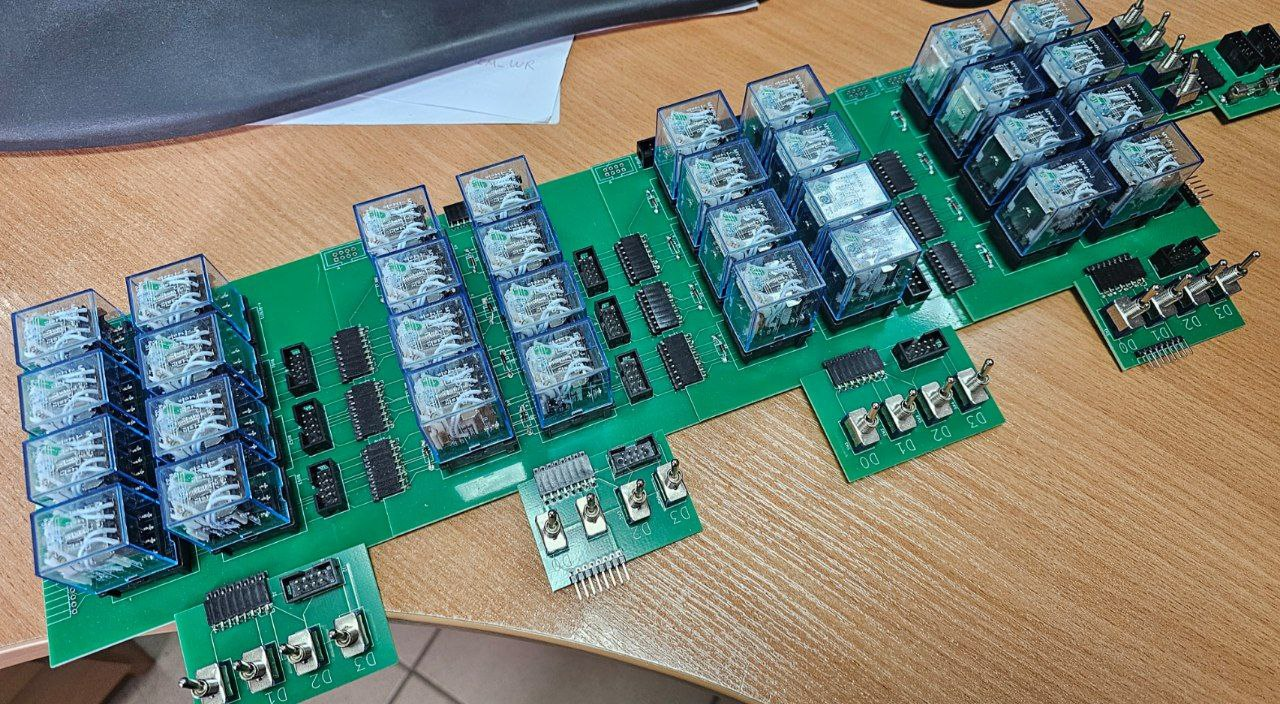
\includegraphics[width=\columnwidth]{photo/register_file.jpg}

Запись в регистры:

\begin{enumerate}
    \item Отключить все управляющие сигналы.
    \item Набрать значение на тумблерах, подключённых к шине данных $1$.
    \item Подключить с помощью тумблера регистр к шине $1$. Убедиться, что в него записалось набранное значение.
    \item Отключить регистр от шины.
    \item Подключить другой регистр к шине $1$. Убедиться, что в него записалось набранное значение.
\end{enumerate}

Копирование значения:

\begin{enumerate}
    \item Отключить все управляющие сигналы.
    \item Подключить регистр с ненулевыми битами к шине $2$.
    \item Подключить пустой регистр к шине $2$. убедиться, что он получил такое же значение, что и в первом регистре.
    \item Отключить все управляющие сигналы.
    \item Аналогично проверить шину $3$.
\end{enumerate}



\chapter{Вычисления}

\section{Логические операции}

\section{Унарные логические операции}

\begin{center}
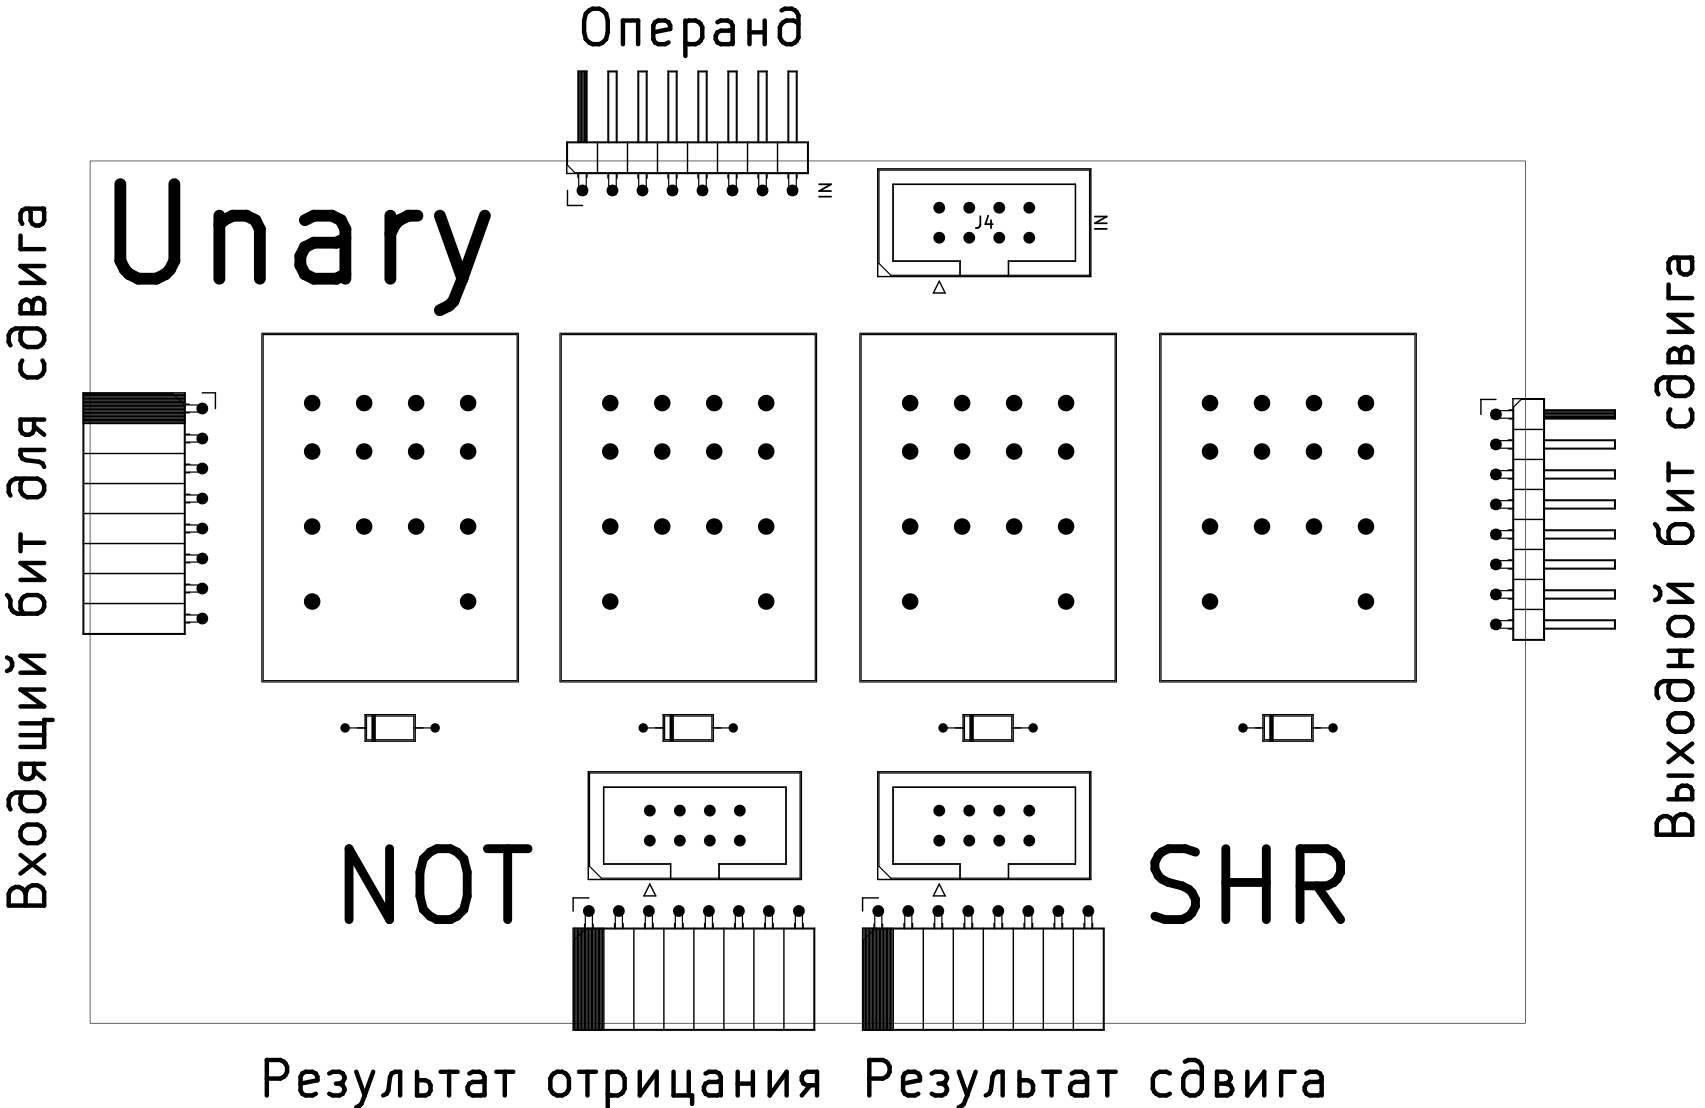
\includegraphics{boards/logic_unary.png}
\end{center}

Модуль для унарных операций выполняет действия над $4$-битным числом: сдвиг вправо и инверсия битов.

Может каскадироваться для сдвига $8$-битных чисел.

\subsection{Практикум}

На вход модуля унарных операций подключается модуль с тумблерами.
Выходы подключаются к шинам регистра.


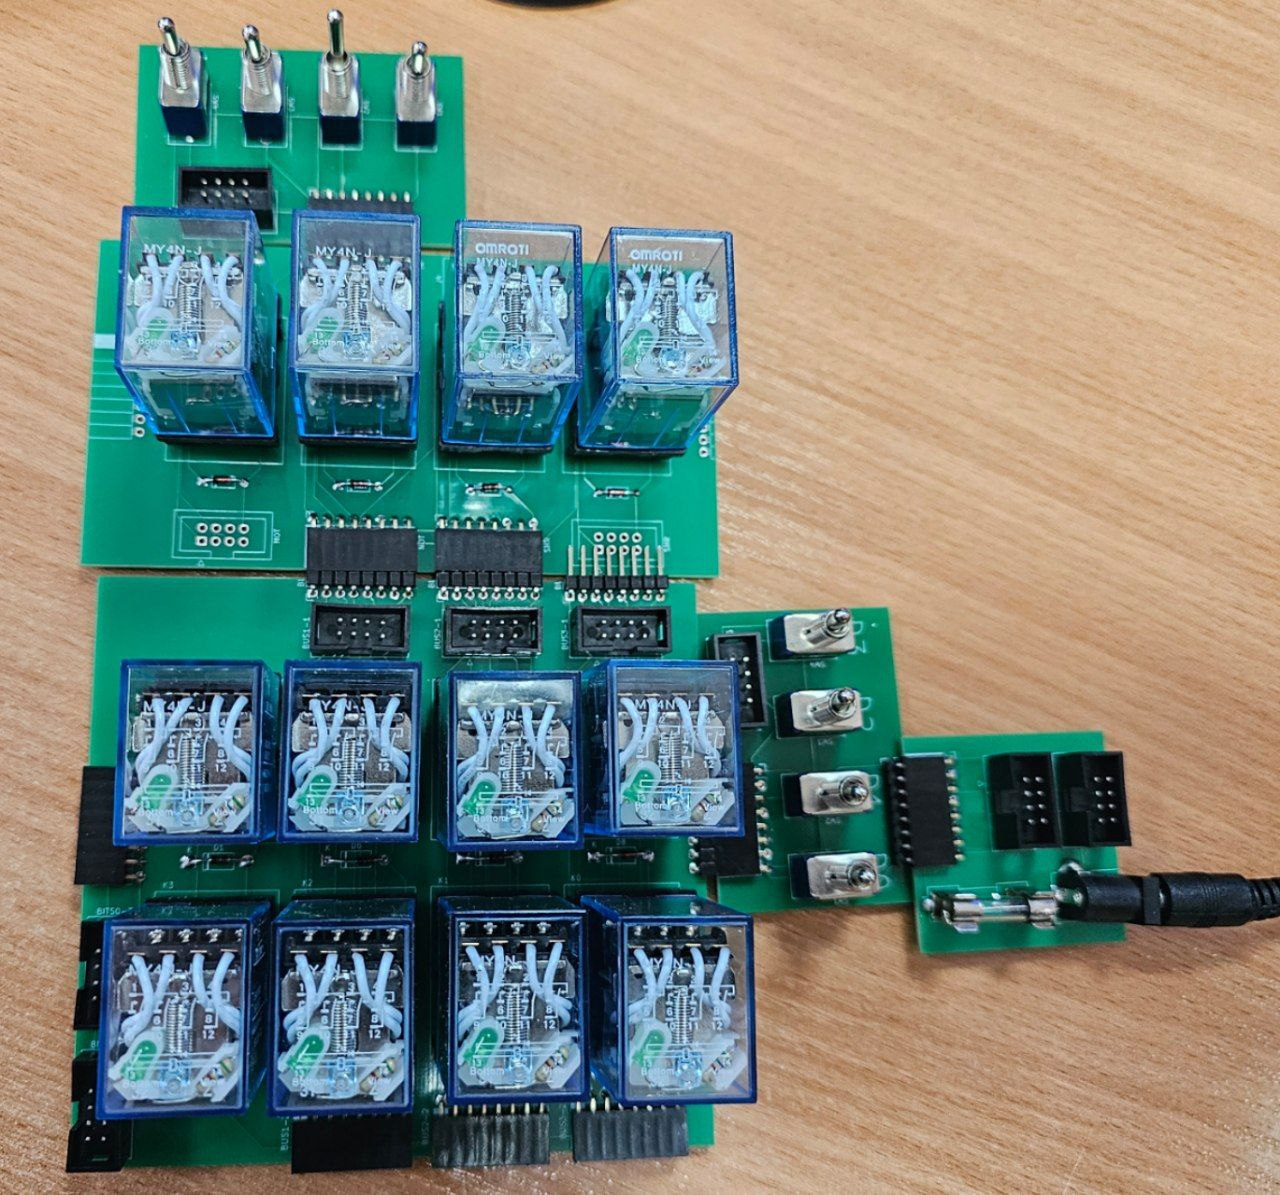
\includegraphics[width=0.5\columnwidth]{photo/unary.jpg}

\begin{enumerate}
    \item Отключить все управляющие сигналы.
    \item Набрать на тумблерах со входными данными значение $1100$.
    \item Подключить выходной регистр к шине $1$. Убедиться, что в него записалось значение $0011$ (инверсия).
    \item Отключить регистр от шины, сбросить его значение.
    \item Подключить выходной регистр к шине $2$. Убедиться, что в него записалось значение $0110$ (сдвиг вправо).
\end{enumerate}

\subsection{Задачи}

\begin{enumerate}
    \item Собрать устройство, позволяющее сдвигать содержимое регистра и записывать результат обратно.
          Занести в регистр значение $1000$ и сдвигать его до тех пор, пока не получится $0001$.
          Вторую часть можно выполнять на скорость.
\end{enumerate}


\section{Логическое И}

Реле представляет собой управляемый выключатель или переключатель.
Если на один контакт $A$ выключателя подать сигнал, то на другом $C$ он появится
только если на обмотке реле $B$ есть напряжение (логическая единица).

\begin{center}
\includegraphics{schemes/and.png}
\end{center}

Получается, что на выходе выключателя сигнал будет только тогда, когда
реле включено и на входе выключателя тоже не ноль. Это означает, что такая
схема реализует операцию логическое <<И>>: $C = A \land B$.



\section{Логическое ИЛИ}


Схему для выполнения логического <<ИЛИ>> можно получить, если соединить два выхода
(две цепи). Тогда напряжение на объединённом выходе появится в любом
из вариантов, если на первом выходе единица или на втором: $C = A \lor B$.

\begin{center}
\includegraphics{schemes/or1.png}
\end{center}

Но у этого способа есть один недостаток. Если на входе $A$ окажется единица,
то так как все входы и выходы соединены в одну цепь, поданное через $A$ напряжение
будет влиять и на вход $B$. И когда $B$ используется ещё где-то,
всё заработает неправильно, какое-то реле включится.
Такой вот паразитный сигнал --- $A$ влияет на выходы, зависящие от $B$.

Поэтому иногда стоит использовать схему с реле для логического <<ИЛИ>>:

\begin{center}
\includegraphics{schemes/or2.png}
\end{center}


\section{Исключающее ИЛИ}

Схема для вычисления <<исключающего или>> несколько сложнее.
Результат операции должен равняться единице только тогда,
когда операнды не равны. То есть если на одном из входов уже
было напряжение, а потом оно появляется и на другом входе,
выход из состояния единицы должен переключиться в ноль.

Такую логику проще всего реализовать с помощью двух переключающих контактов:

\begin{center}
\includegraphics{schemes/xor.png}
\end{center}

Благодаря перекрёстному соединению переключателей проводниками,
сигнал на выходе $C$ появляется только тогда, когда переключатели на реле
находятся в противоположных положениях.

\section{Бинарные логические операции}

\begin{center}
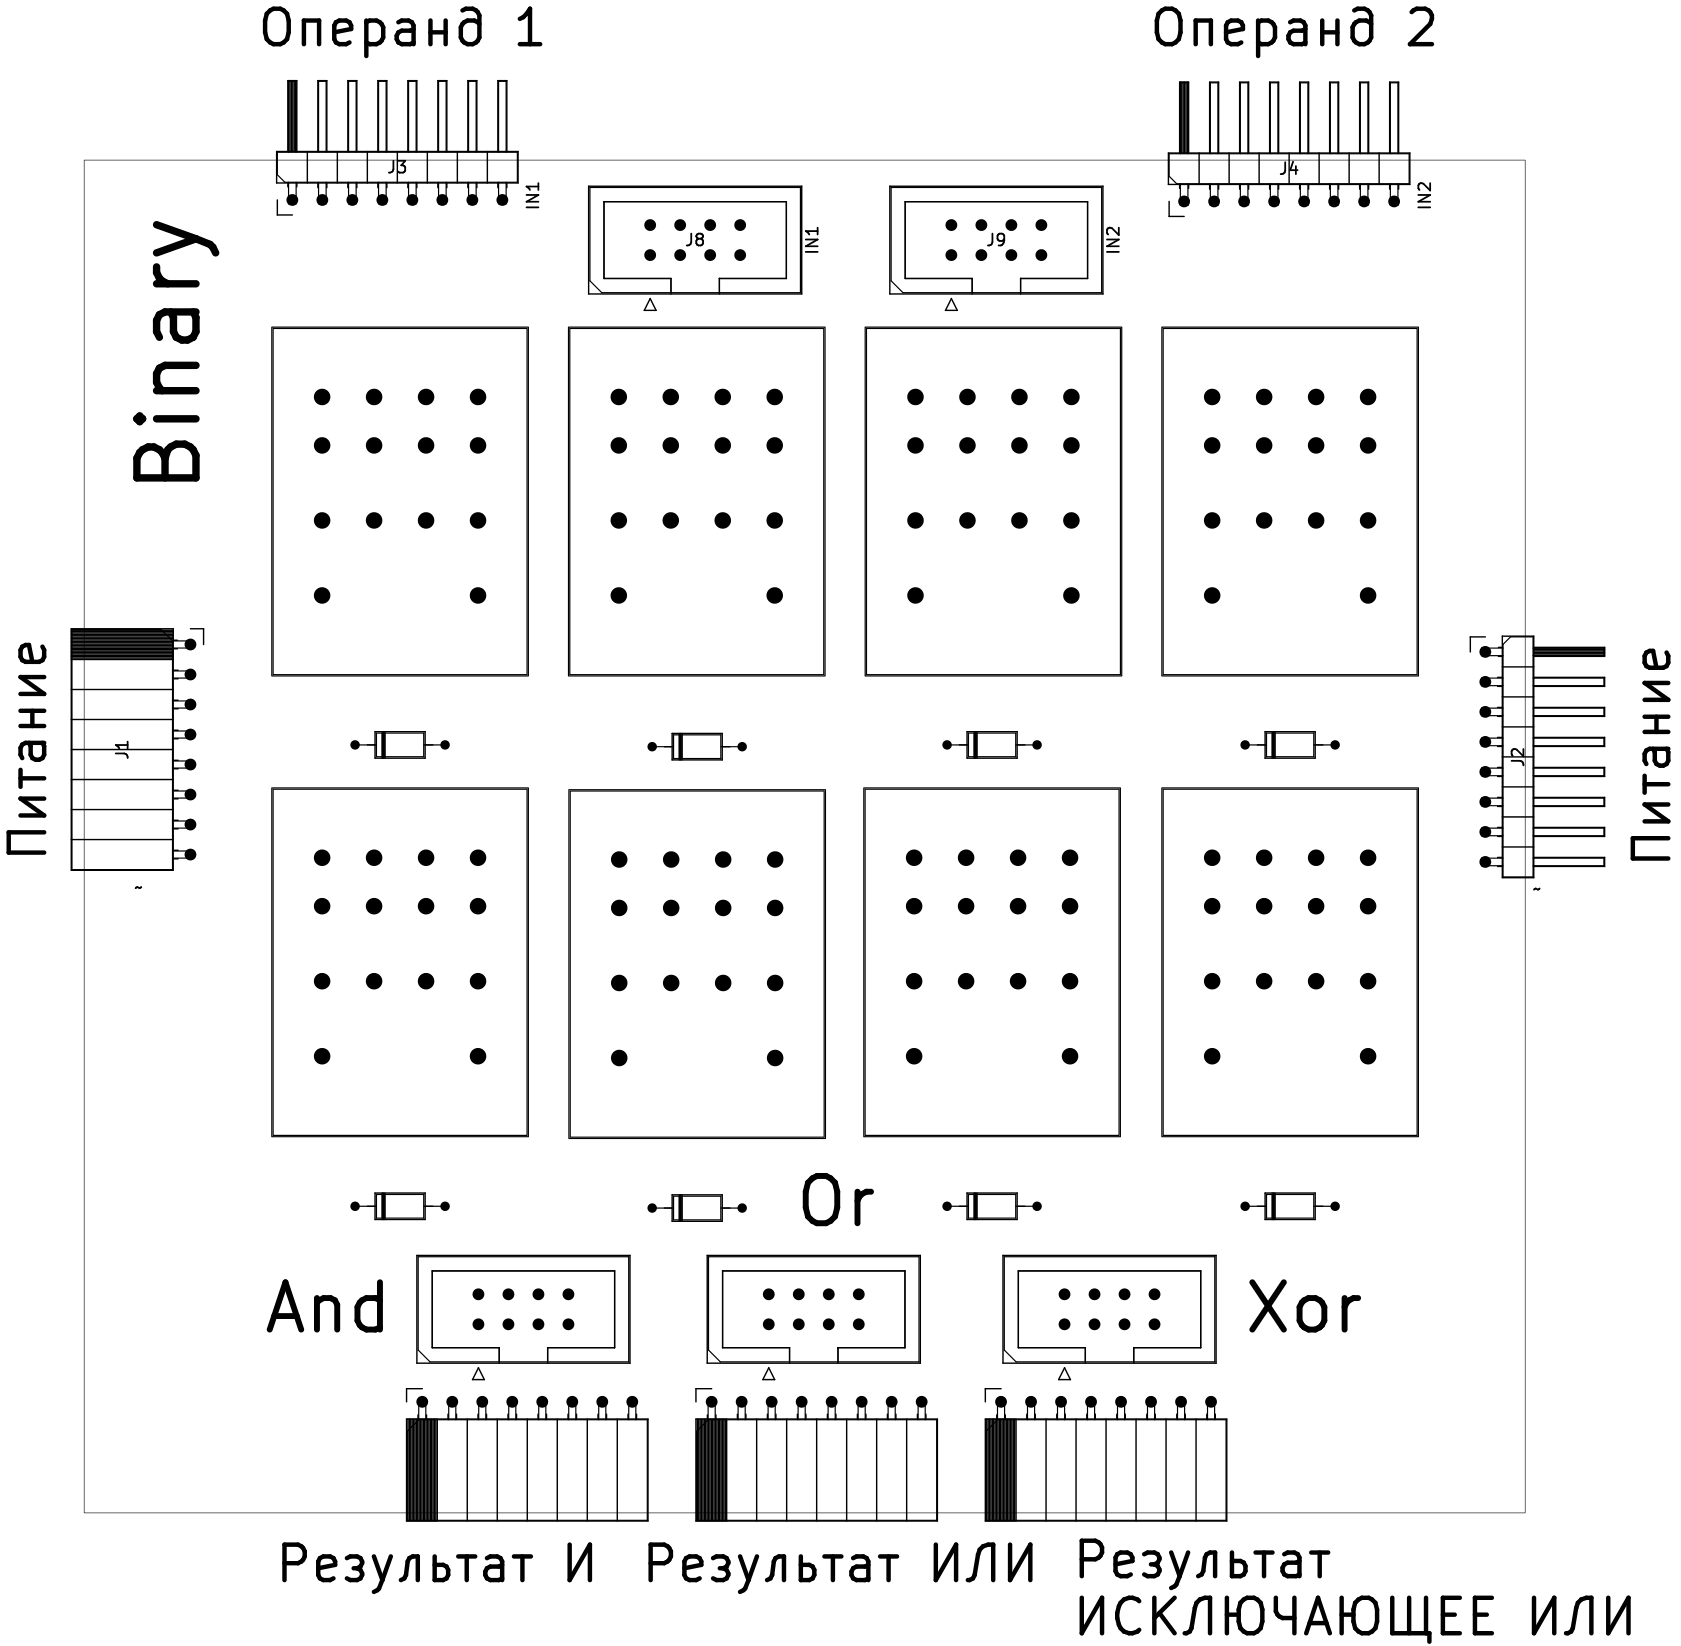
\includegraphics{boards/logic_binary.png}
\end{center}

Модуль логических операций поддерживает вычисление AND, OR и XOR.
У модуля есть два четырёхбитных входа и три выхода.
Каждый выход отвечает за одну операцию.

\subsection{Подготовка}

\begin{enumerate}
    \item Как могла бы выглядеть схема для выполнения операцию XOR?
\end{enumerate}

\subsection{Практикум}

Ко входам модуля подключаются два модуля с тумблерами, а к выходам --- регистр,
куда будет записываться результат.


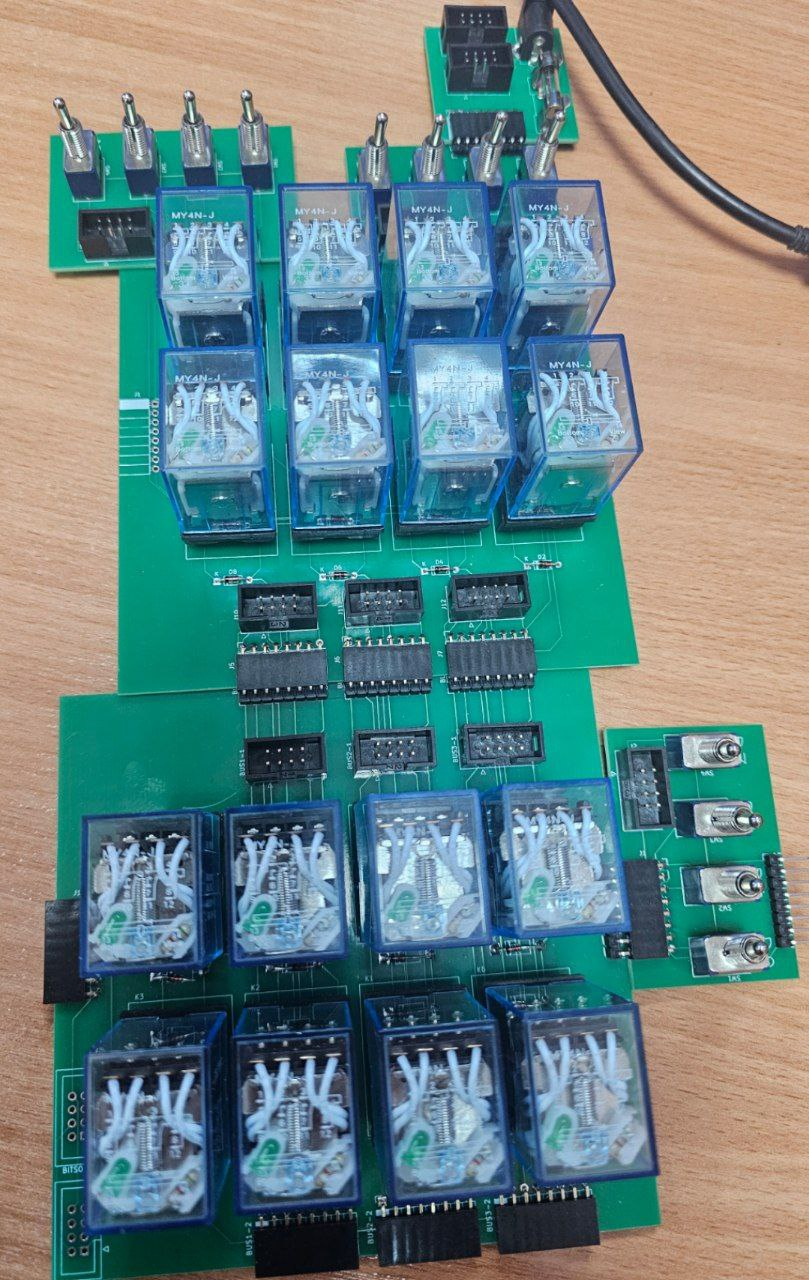
\includegraphics[width=0.5\columnwidth]{photo/logic.jpg}

\begin{enumerate}
    \item Отключить все управляющие сигналы.
    \item Набрать на тумблерах первого операнда значение $1100$.
    \item Набрать на тумблерах второго операнда значение $1010$.
    \item Подключить выходной регистр к шине $1$. Убедиться, что в него записалось значение $1000$ (AND).
    \item Отключить регистр от шины, сбросить его значение.
    \item Подключить выходной регистр к шине $2$. Убедиться, что в него записалось значение $1110$ (OR).
    \item Отключить регистр от шины, сбросить его значение.
    \item Подключить выходной регистр к шине $3$. Убедиться, что в него записалось значение $0110$ (XOR).
\end{enumerate}




\section{Шина и регистровый файл}

Несколько регистров можно соединить в регистровый файл.
У каждого из регистров есть сигналы выборки на одну из трёх шин.

Если два регистра подключены к одной шине одновременно,
то значения одного будут копироваться в другой. Если точнее,
включённые биты включают аналогичные в другом регистре, то есть
копирование возможно в обе стороны одновременно.

Нулевые биты при этом копироваться не могут. Для записи нулей
регистр необходимо сбросить.


\subsection{Практикум}


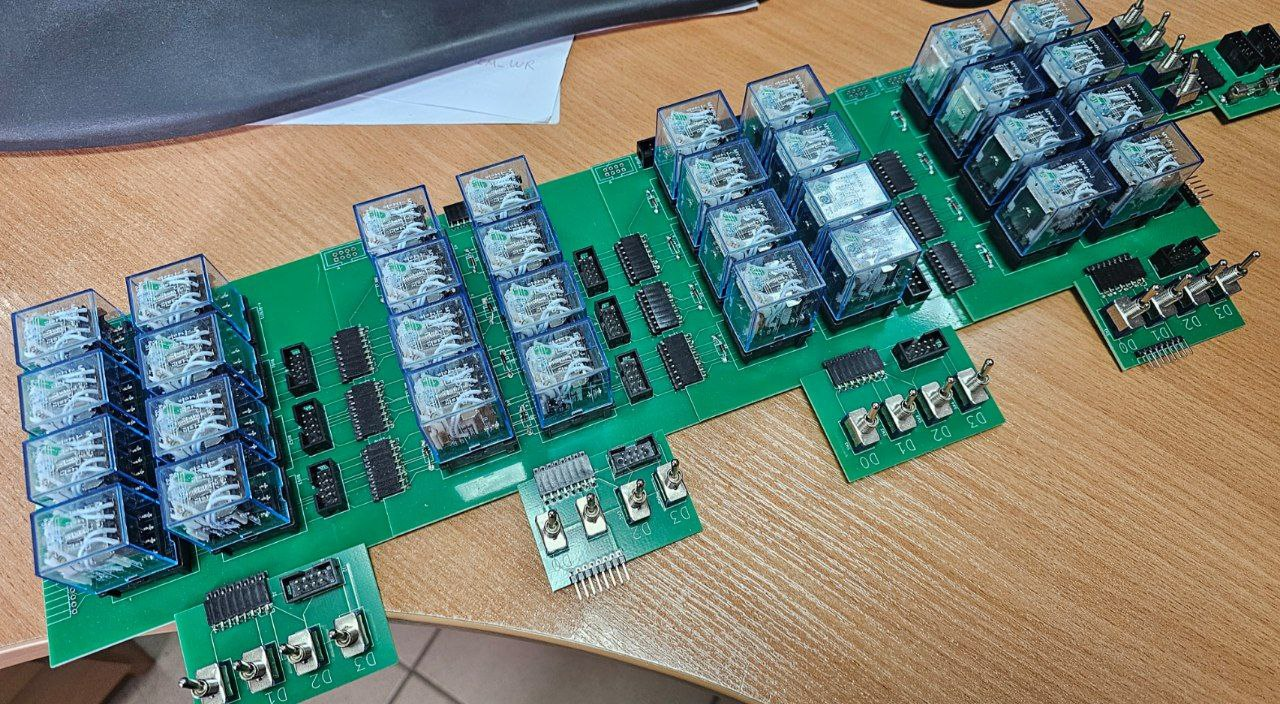
\includegraphics[width=\columnwidth]{photo/register_file.jpg}

Запись в регистры:

\begin{enumerate}
    \item Отключить все управляющие сигналы.
    \item Набрать значение на тумблерах, подключённых к шине данных $1$.
    \item Подключить с помощью тумблера регистр к шине $1$. Убедиться, что в него записалось набранное значение.
    \item Отключить регистр от шины.
    \item Подключить другой регистр к шине $1$. Убедиться, что в него записалось набранное значение.
\end{enumerate}

Копирование значения:

\begin{enumerate}
    \item Отключить все управляющие сигналы.
    \item Подключить регистр с ненулевыми битами к шине $2$.
    \item Подключить пустой регистр к шине $2$. убедиться, что он получил такое же значение, что и в первом регистре.
    \item Отключить все управляющие сигналы.
    \item Аналогично проверить шину $3$.
\end{enumerate}



\section{Арифметические операции}

\section{Сложение}

Чтобы складывать числа, сначала нужно научиться складывать отдельные биты.
Сумма двух битов может дать результат $0_2$, $1_2$ или $10_2$.
То есть при сложении получается уже двухбитовое число.

Схему сложения удобнее всего строить из однотипных компонентов, складывающих
фиксированное количество битов. На выходе такого компонента будет результат
сложения, а также бит переполнения (переноса). Для каскадирования
таких модулей нужно также иметь возможность подавать на вход перенос от
сумматоров младших битов.

Таким образом, сумматор получает на вход бит переноса и два числа, а на выходе
у него тоже бит переноса и число-сумма.


\section{Сумматор}

\begin{center}
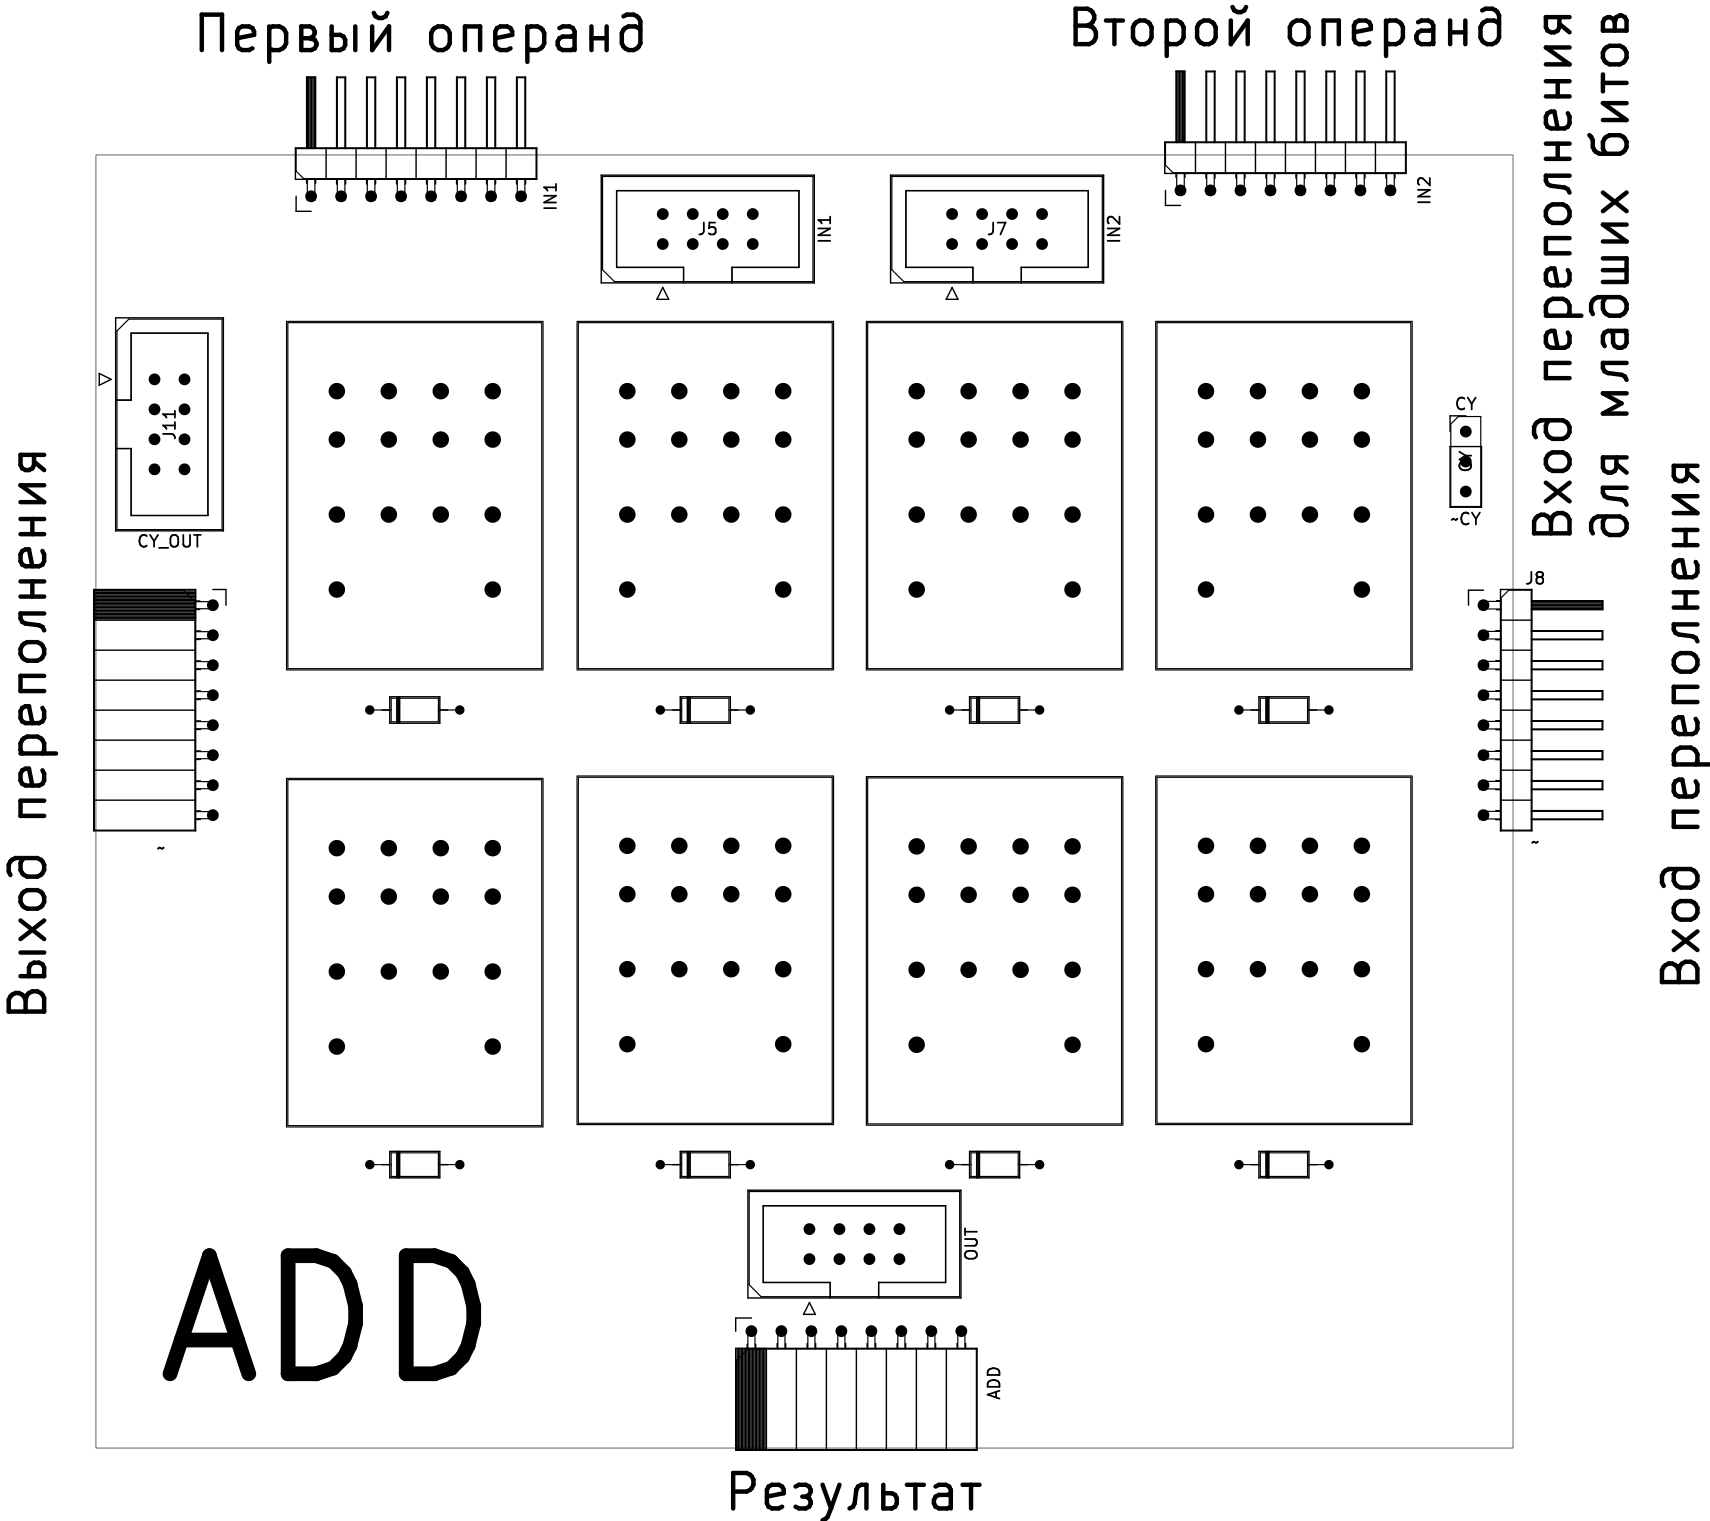
\includegraphics{boards/adder.png}
\end{center}

Сумматор складывает два четырёхбитных числа, один бит переноса и выдаёт четырёхбитное число и бит переноса.
У модуля есть два четырёхбитный вход и один выход.
Каждый выход отвечает за одну операцию.


\subsection{Подготовка}

\begin{enumerate}
    \item Придумайте, как можно было бы составить схему из реле, чтобы вычислять сумму однобитовых чисел.
    \item Как можно использовать предыдущую схему для вычисления суммы двухбитовых чисел?
\end{enumerate}

\subsection{Практикум}

Ко входам модуля подключаются два модуля с тумблерами, а к выходам --- регистр,
куда будет записываться результат.

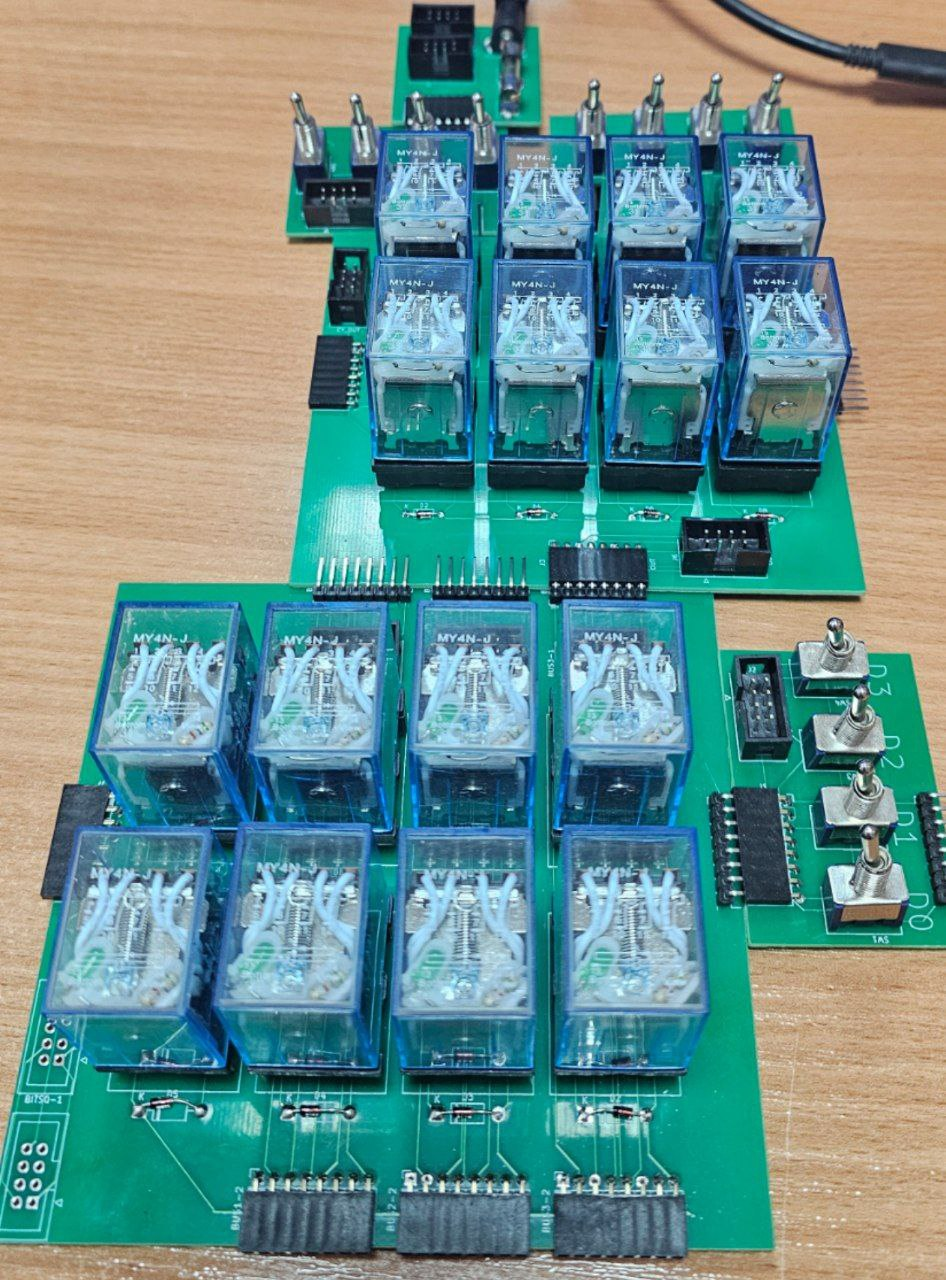
\includegraphics[width=0.5\columnwidth]{photo/adder.jpg}

\begin{enumerate}
    \item Отключить все управляющие сигналы.
    \item Установить перемычку для подачи сигнала на $~CY$.
    \item Набрать на тумблерах первого операнда значение $0011$ (число $3$).
    \item Набрать на тумблерах второго операнда значение $1010$ (число $10$).
    \item Подключить выходной регистр к шине $3$. Убедиться, что в него записалось значение $1101$ (число $13$).
    \item Отключить регистр от шины, сбросить его значение.
    \item Установить перемычку для подачи сигнала на $CY$.
    \item Подключить выходной регистр к шине $3$. Убедиться, что в него записалось значение $1110$ (число $14$).
\end{enumerate}


\subsection{Задачи}

\begin{enumerate}
    \item Собрать устройство для сложения значения из регистра с константой, набранной на тумблерах.
          Должна быть предусмотрена запись результата обратно в регистр.
          Дальше управлять сигналами таким образом, чтобы к регистру последовательно
          прибавлялась единица, пока он не достигнет значения $1111$.
\end{enumerate}



\section{Вычитание}

\subsection{Вычитание через сложение с дополнительным обратным кодом}

Чтобы вычесть из одного числа другое, можно вычитаемое представить в дополнительном обратном
коде, а затем сложить это число с уменьшаемым.

Число в дополнительном обратном коде получается, если сначала инвертировать биты исходного
числа, а затем прибавить к нему единицу.

Например, для числа $3=0011$ инверсия будет выглядеть, как $1100$, а дополнительный обратный код, как $1101$.

\subsubsection{Практикум}

Собрать схему для сложения.

\begin{enumerate}
    \item Отключить все управляющие сигналы.
    \item Установить перемычку для подачи сигнала на $~CY$.
    \item Набрать на тумблерах первого операнда значение $1010$ (число $10$).
    \item Набрать на тумблерах второго операнда значение $1101$ (число $-3$).
    \item Подключить выходной регистр к шине $3$. Убедиться, что в него записалось значение $0111$ (число $7$).
\end{enumerate}

\subsubsection{Задачи}
\begin{enumerate}
    \item Выполните деление в столбик числа $14$ на $3$ с помощью последовательности вычитаний.
          Записывайте промежуточные результаты на бумаге.
    \item Сделайте то же самое, только сохраняйте все промежуточные результаты в разных
          регистрах регистрового файла.
\end{enumerate}

\subsection{Вычитание с помощью сумматора и инвертора}

Вычитание можно делать с помощью сумматора. Чтобы на входе из операнда получался дополнительный
обратный код, сначала нужно преобразовать его с помощью инвертора, а затем прибавить $1$,
включив вход переноса в сумматоре.

\subsubsection{Практикум}

Собрать схему для сложения, а затем добавить между тумблерами со вторым операндом
инвертор (выход NOT блока унарной логики):

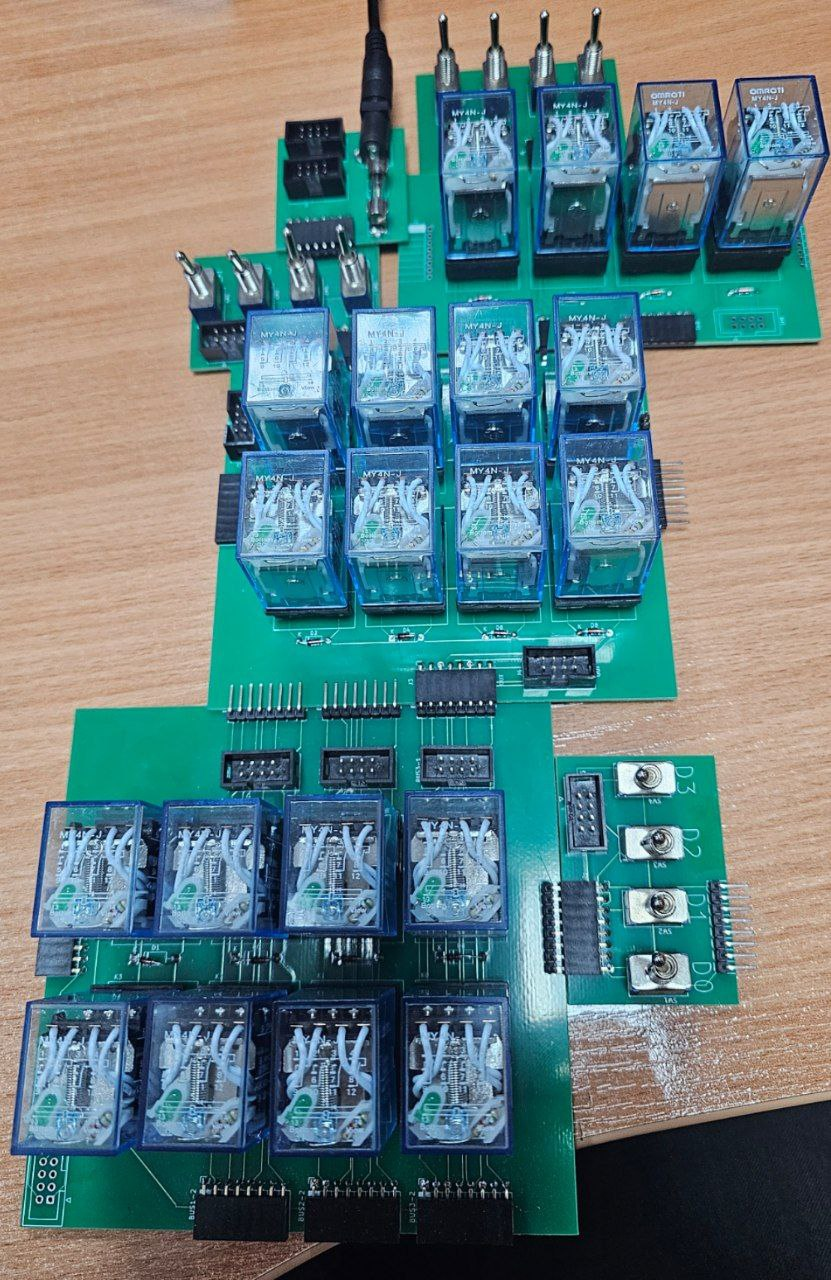
\includegraphics[width=0.5\columnwidth]{photo/subtractor.jpg}

\begin{enumerate}
    \item Отключить все управляющие сигналы.
    \item Установить перемычку для подачи сигнала на $CY$.
    \item Набрать на тумблерах первого операнда значение $1010$ (число $10$).
    \item Набрать на тумблерах второго операнда значение $0011$ (число $3$).
    \item Подключить выходной регистр к шине $3$. Убедиться, что в него записалось значение $0111$ (число $7$).
\end{enumerate}

\chapter{Калькулятор}

\section{Чем калькулятор отличается от компьютера?}


\section{Калькулятор для 7 операций}

Все вычислители можно соединить с одним и тем же регистром, как хранилищем результата, чтобы получить простейший
калькулятор. Доступны следующие операции:
\begin{enumerate}
    \item Инверсия
    \item Сдвиг вправо
    \item Побитовое И
    \item Побитовое ИЛИ
    \item Исключающее ИЛИ
    \item Сложение
    \item Вычитание
\end{enumerate}

\subsubsection{Практикум}

Список модулей:
\begin{itemize}
    \item Модуль переключателей: $10$ штук
    \item Модуль унарных операций: $2$ штуки
    \item Сумматор: $2$ штуки
    \item Модуль логических операций: $1$ штука
    \item Регистровый модуль как шинный формирователь: $2$ штуки
    \item Регистровый модуль: $1$ штука
    \item Модуль шины: $1$ штука
    \item Соединительные шлейфы: $4$ штуки
\end{itemize}

Уже проверенные модули для разных операций соединяются вместе.
Для этого используются несколько мультиплексоров (шинных формирователей)
на платах регистров. На этих платах не установлены реле для хранения
битов. Вместо этого шины подключаются к одному и тому же регистру.
Так в него можно записывать любой из $7$ результатов вычислений.

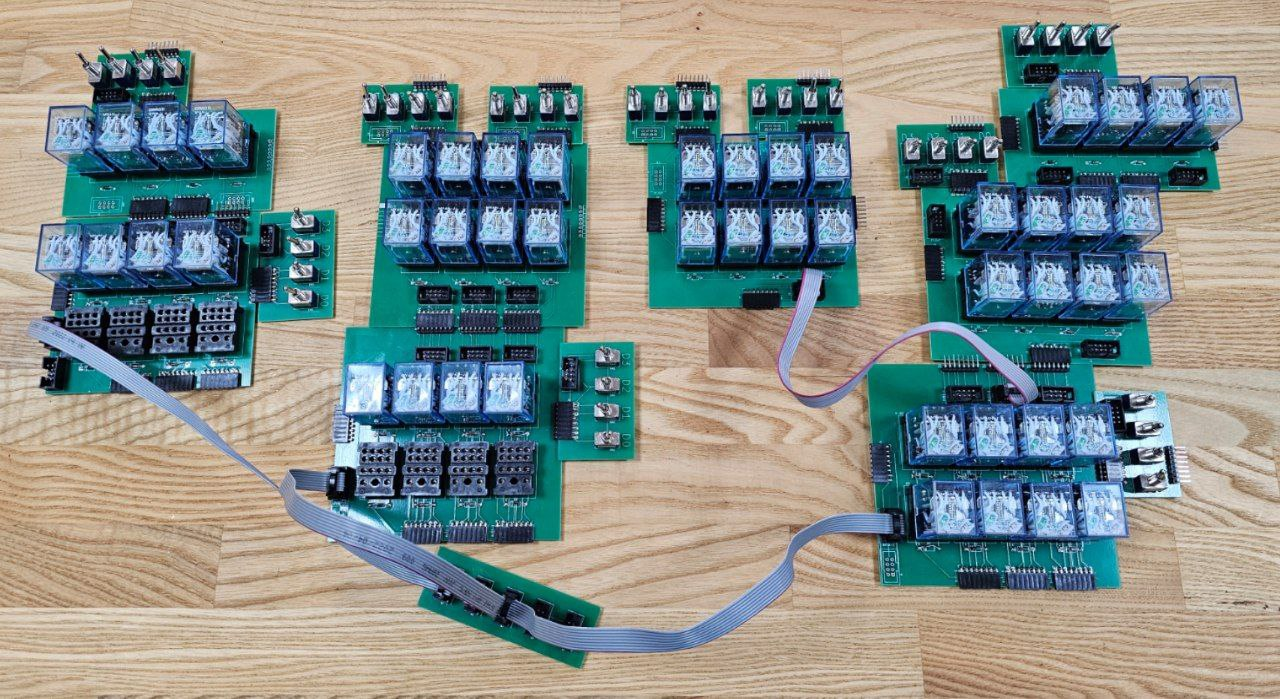
\includegraphics[width=\columnwidth]{photo/calculator.jpg}

Любую из операций можно выполнить так:

\begin{enumerate}
    \item Отключить все управляющие сигналы.
    \item Набрать входные данные для нужной операции.
    \item Подключить выход нужного модуля к регистру тумблером.
    \item Наблюдать результаты вычислений.
    \item Сбросить значение регистра.
\end{enumerate}


\section{Расширение вычислений до восьми бит}

У регистров и вычислительных модулей справа и слева есть разъёмы для расширения разрядности.

Для регистров через эти разъёмы передаются сигналы сброса и подключения к шинам. Поэтому
один набор тумблеров может использоваться для двух четырёхбитных плат-регистров, если они
соединены в один восьмибитный регистр.

Для вычислительных модулей через боковые разъёмы передаются сигналы переноса (в случае сдвига и сложения).

\subsubsection{Практикум}

Соединить два регистра и два сумматора. Шина $3$ регистров подключается к сумматору.
У правого (младшего) сумматора входящий перенос перемычкой устанавливается в $0$.
У левого (старшего) сумматора перемычка для переноса убирается, потому что
сигнал переноса приходит от младших битов (из правого сумматора).

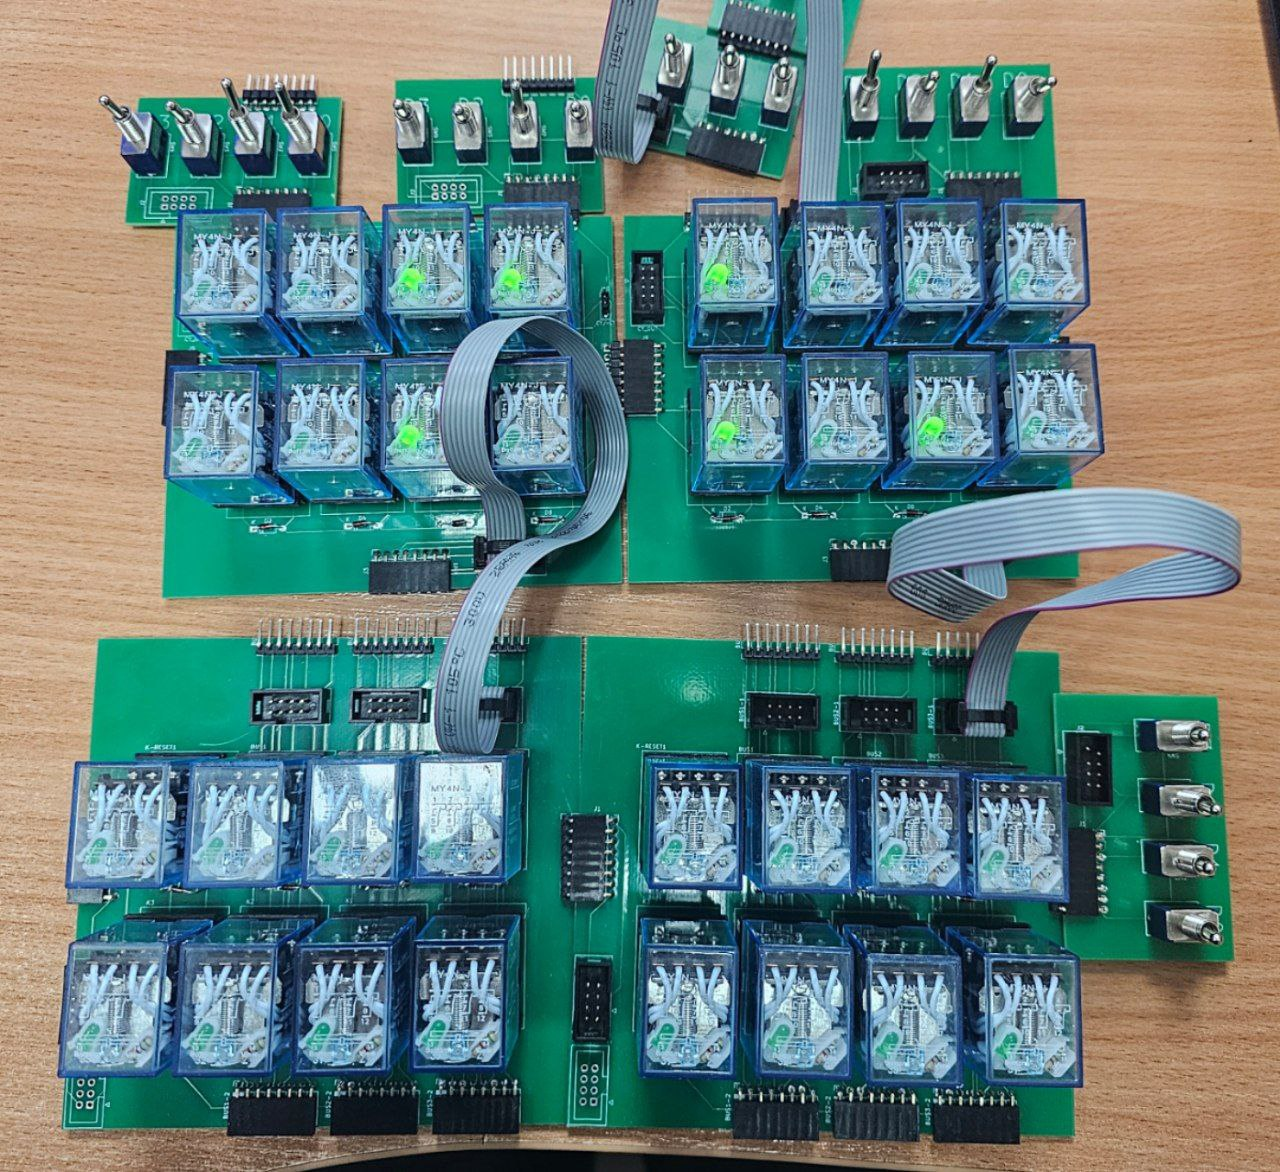
\includegraphics[width=0.5\columnwidth]{photo/8bit.jpg}

\begin{enumerate}
    \item Отключить все управляющие сигналы.
    \item Набрать входные данные $0011 1001$ и $0010 1001$.
    \item Подключить выход сумматора к регистру тумблером $D3$.
    \item Наблюдать результат вычислений $0110 0010$.
\end{enumerate}





\chapter{Элементы компьютера}

\section{Дешифратор}

\section{ПЗУ}

\section{Декодер инструкций}

\section{Тактовый генератор}


\chapter{Компьютер}

\end{document}
